\subsubsection{Query Transformation}
The aim of this section is to study some properties of $(u,v)$-mincut which help us to transform a query procedure to another equivalent query. Remember, the query we have is of the form $Q(u,v,E_y)$ on graph $G$ in which we need to report if all edges in $E_y$ lie in some $(u,v)$-mincut. Another set of edges from graph $G$, say $E'$, not necessarily having common end point is obtained, which satisfies the property that all edges in $E_y$ lie in some $(u,v)$-mincut if and only if all edges in $E'$ lie in some $(u,v)$-mincut.

One might question the relevance of such a transformation for our use. We will make use of this transformation to get a set of edges $E'$ which have the following property,
~(i) their endpoints are different vertices in $G_\nu$, and
~(ii) all the edges in $E'$ share a common end point in $G_\nu$. This will enable us to transform a query $Q(u,v,E_y)$ on $G$ to an equivalent query $Q(u,v,E')$ on $G_\nu$.

% {\color{red} SODA2021-alternate import begin}

%%%%%%%Query transformation lemma begin

Let $r,s,t$ be any three vertices from $S$
and let $A\subset V$ define a steiner mincut that separates $\{r,s\}$ from $t$. Recall that strip ${\cal W}_A$ stores all $(s,t)$-mincuts that enclose $A$. Our aim is to investigate the properties of a $(r,s)$-mincut with respect to the strip ${\cal W}_A$.

Let $B$ be any $(r,s)$-mincut. If $B\subseteq A$, all vertices presents in the nodes ${\cal W}_A\backslash {\mathbf{s}}$ appear on one side of the $(r,s)$-mincut. So let us consider the more interesting case in which $B$ crosses $A$. Firstly, it follows from Lemma \ref{lem:B-crosses-A} that each node of the strip ${\cal W}_A$, excluding of course $\mathbf{s}$, remain intact in each $(r,s)$-mincut. This suggests that we can replace the subgraph of $G$ induced by $\bar{A}$ by the strip ${\cal W}_A$ above ${\mathbf{s}}$. Alternatively, we blow-up the node $\mathbf{s}$ of ${\cal W}_A$ into the subgraph induced by the vertices assigned to it. We call this graph $G_A$ henceforth. The following figure illustrates ${\cal W}_A$ and $G_A$.

\begin{figure}[h]
    \centering
    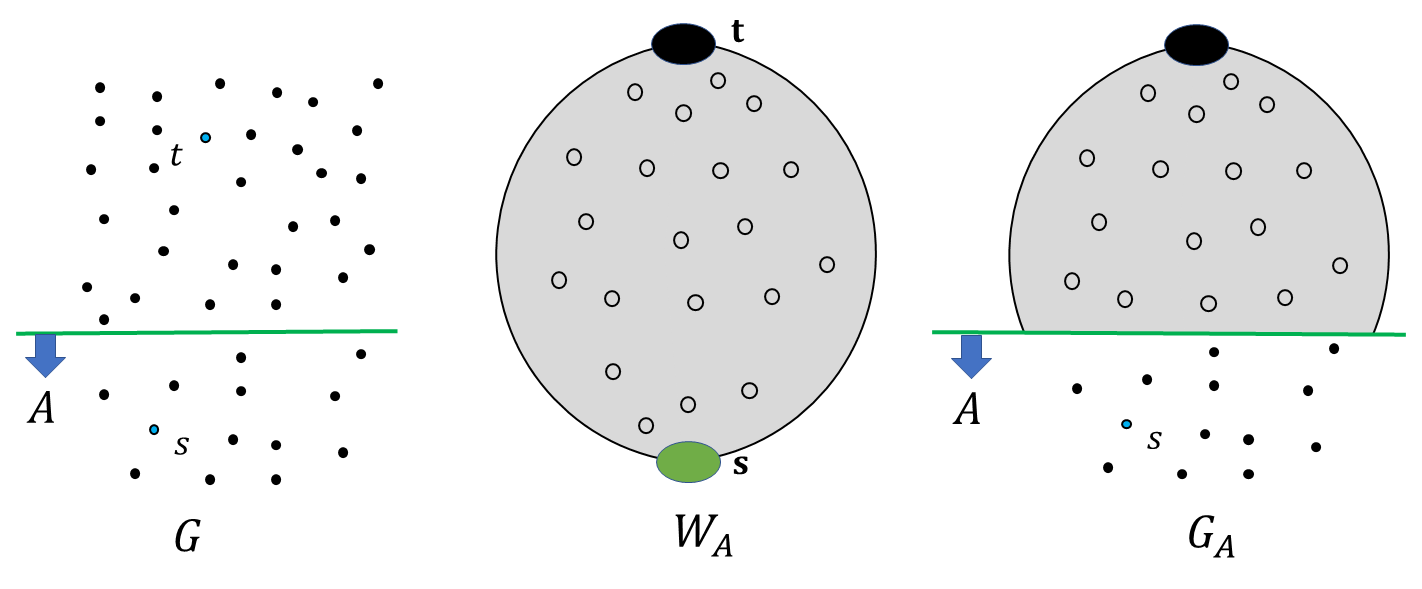
\includegraphics[width=0.9\textwidth]{src/images/G_A.png}{}
    \caption{Suitable caption to be added}
    \label{fig:G_A}
\end{figure}

Let $y$ be any non-terminal unit in strip ${\cal W}_{A}$. Let $x_1,\ldots,x_k$ be any $k$ neighbors of $y$. In case all the neighbours are on the side of $\mathbf{s}$, let $R$ be the union of their reachability cones, on the side of $\mathbf{s}$, excluding the terminal ${\mathbf{s}}$. In case all neighbours are on the side of $\mathbf{t}$, consider $R$ to be the reachability cone of $y$ on the side of $\mathbf{s}$ excluding the terminal $\mathbf{s}$.

We know that there exists a $(s,t)$-mincut that cuts edges $(y,x_i)$ for each $1\le i \le k$. There also exists a $(s,t)$-mincut that cuts all edges emanating from $R$ on the side of $\mathbf{s}$. What about the $(r,s)$-cut defined by $B$ that crosses $A$. We shall show an important claim on the following page. The intuition underlying the claim is as follows. 

For each $(r,s)$-cut that crosses $A$, we can associate a $(r,t)$-mincut that encloses $A$. Since the latter is a transversal on ${\cal W}_A$, this allows us to exploit properties of ${\cal W}_A$ stated in 
Lemma \ref{lem:reachability-cone-in-W-st} and Corollary
\ref{cor:1-W_A-2-nearest-mincut}. This helps us in deriving inferences for the cut defined by $B$.

\begin{lemma}
\label{lem:reachability-cone-u-v-mincut}
There is a $(r,s)$-mincut that cuts edges $\{(y,x_1),\ldots, (y,x_k)\}$ if and only if there is a $(r,s)$-mincut that cuts all edges emanating from $R$ on the side of $\mathbf{s}$.
\end{lemma}
\begin{proof}
Let all $x_i's$ be on the side of $\mathbf s$ from $y$. The proof for other side will follow likewise.

Let $B$ be a $(r,s)$-mincut that cuts edges $\{(y,x_1),…,(y,x_k)\}$. 
Refer to Figure \ref{fig:B-crosses-A}($i$).
Observe that $y$ does not belong to $A$. So $A\cup B$ also cuts edges $\{(y,x_1),…,(y,x_k)\}$, and $\{x_1,\ldots,x_k\}$ belong to $A\cup B$.
It follows from  Lemma \ref{lem:B-crosses-A} (ii) that $A\cup B$ is a $(r,t)$-mincut. Since $A\cup B$ encloses $A$, so
$A\cup B$ must be a transversal on ${\cal W}_A$.  Therefore,
$R$ belongs to $A\cup B$.
%Applying Corollary \ref{cor:1-W_A-2-nearest-mincut}(2), it follows that the nearest mincut between $\{r,x_1,…,x_k\}$ and $t$ must contain $R$. 
%Since $x_i$’s belong to $A\cup B$, it follows that $A\cup B$ is also a mincut between $\{r ,x_1,…,x_k\}$  and $t$. 
%So $R$ belongs to $A\cup B$ as well.
It follows from the construction that $R$ lies totally outside $A$, that is, $R\cap A=\emptyset$. Therefore, since
$R$ belongs to $A\cup B$, $R$ must lie fully inside $\bar{A}\cap B$. 
Using this fact and Lemma \ref{lem:B-crosses-A} (iii), all edges emanating from $R$ on the side of $\mathbf{s}$
are incident only on $A\cap B$. But $A\cap B$ defines a $(r,s)$-mincut as follows from Lemma \ref{lem:B-crosses-A} (i). 
%This cut is obtained by removing $\bar{A}\cap B$ from $B$. So it follows that $R$ lies outside $A\cap B$ and $R$ contributes all outgoing edges to the cut defined by $A\cap B$. 
So $A\cap B$ defines the desired $(r,s)$-cut.
\begin{figure}[h]
    \centering
    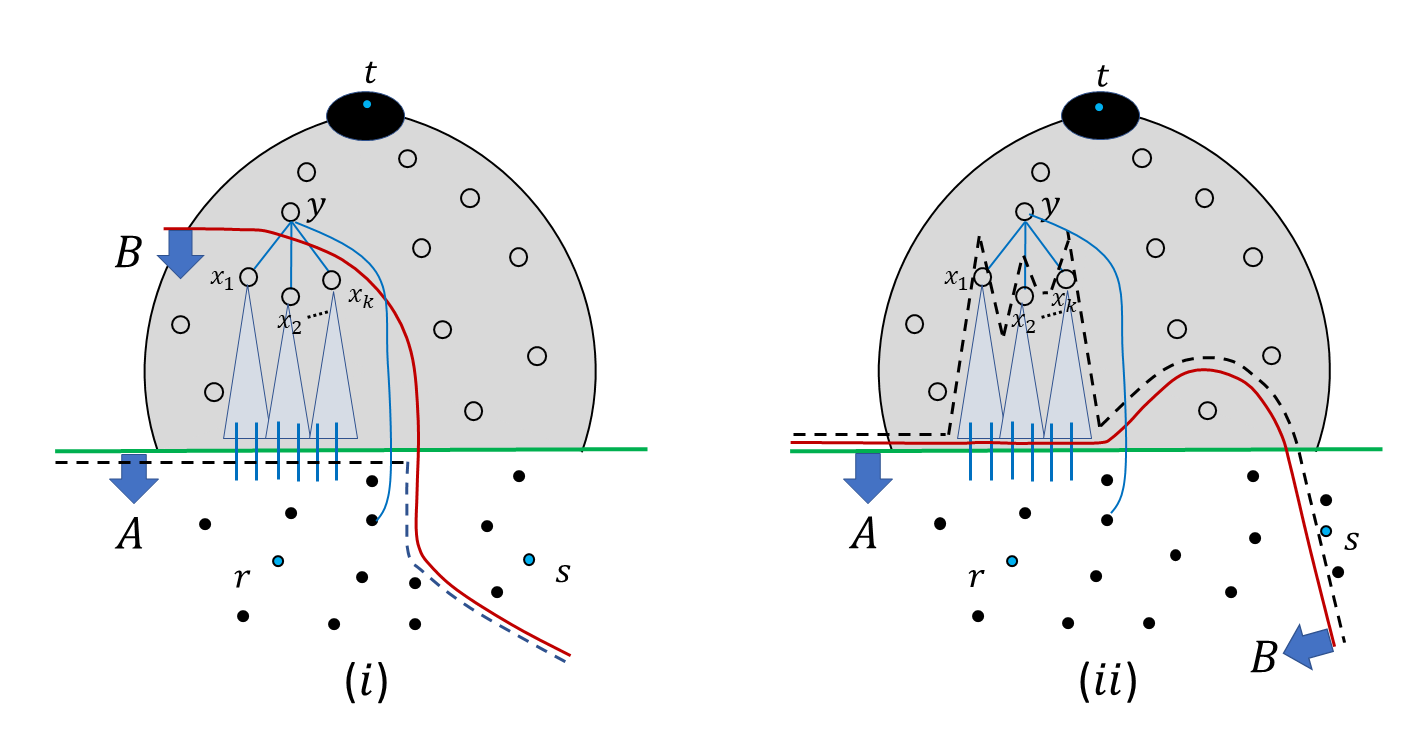
\includegraphics[width=0.9\textwidth]{src/images/B-crosses-A.png}{}
    \caption{($i$) $B$ cuts edges $\{(y,x_1),\ldots,(y,x_k)\}$.~$(ii)$ $B$ cuts all outgoing edges of $R$.}
    \label{fig:B-crosses-A}
\end{figure}

Let $B$ be a $(r,s)$-mincut with that cuts all edges emanating from $R$ on the side of $\mathbf{s}$. Refer to Figure \ref{fig:B-crosses-A}($ii$). By construction $R$ lies outside $A$, and the cut defined by $A$ cuts all edges emanating from $R$ on the side of $\mathbf{s}$.
 Therefore, the cut defined by $A\cup B$ cuts all edges emanating from $R$ on the side of $\mathbf{s}$. Using Lemma \ref{lem:B-crosses-A} (ii), $A\cup B$ is a $(r,t)$-mincut. Since each $(r,t)$-mincut that encloses $A$ is a transversal on ${\cal W}_A$, it follows that $(A\cup B) \cap R = \emptyset$. So $B \cap R = \emptyset$ too. That is, $R$ lies entirely on the side of $t$ in the cut defined by $B$. Treating $R$ as a single vertex, observe that its incoming edges are the same in number as its outgoing edges. It is given that $R$ currently contributes all its outgoing edges to the cut defined by $B$. So it follows that $B\cup R$ has the same capacity as $B$ and $R$ now contributes all incoming edges to the cut defined by $B \cup R$. Now observe that $r$ belongs to $B\cup R$ since $r$ is in $B$ by construction. $s$ does not belong to $B \cup R$ since, by construction, $s$ is neither in $R$ nor in $B$. So  $B\cup R$ is a $(r,s)$-mincut. It follows from above that all incoming edges of $R$ contribute to this cut. So the cut defined by $B\cup R$ cuts all edges $(y,x_1),…,(y,x_k)$. So $B\cup R$ is the desired $(r,s)$-cut.
\end{proof}

%%%% Query transformation lemma end %%%%
% {\color{red} SODA2021-alternate import end}




\subsection{Construction of compact graph for any $S\subseteq V$}
{\color{red} Correct cycles to cycles/tree edges}
The contraction procedure is pretty much the same as in the contraction at root node. The only difference is caused by stretched units as they are mapped to a proper path in the skeleton ${\cal H}_S$ rather than a single node. The construction of $G_\nu$ is as follows.

Let us fix any arbitrary total order on the cycles and tree edges in skeleton ${\cal H}_S$. It is important to note that the ordering is same for cycles and tree edges. The construction of $G_\nu$ is as follows. We keep all the vertices mapped to node $\nu$ in the skeleton as it is in $G_\nu$ (call them $V_\nu$). We create $j = |C_\nu|+|E_\nu|$ vertices, one for each of the $j$ cycles and tree-edges in the set $C_\nu \cup E_\nu$. Since, we have a total order on all cyles and tree edges. We can assume that $C_\nu \cup E_\nu$ is an ordered set. The $\ell^{th}$ element of this set be denoted by $e_\ell$. Let $c_\ell$ denote the vertex corresponding to $e_\ell$. Consider any vertex $v\notin V_\nu$. Let the unit, it belongs to, be mapped to  $P(\nu_1,\nu_2)$. We assign $v$ to one of $\{c_1,\ldots,c_j\}$ as follows.
\begin{itemize}
    \item If $\nu_1=\nu$ and $\nu_2\in {\cal H_S}(e_i)$, $v$ is assigned to $c_i$. Moreover, if  $\nu_1\in {\cal H_S}(e_i)$ and $\nu_2=\nu$, $v$ is assigned to $c_i$.
    \item If $\nu_1 \in {\cal H_S}(e_i)$ and $\nu_2\in {\cal H_S}(e_k)$, $v$ is assigned to $c_{\min(i,k)}$
\end{itemize}

\noindent

\begin{figure}[h]
    \centering
    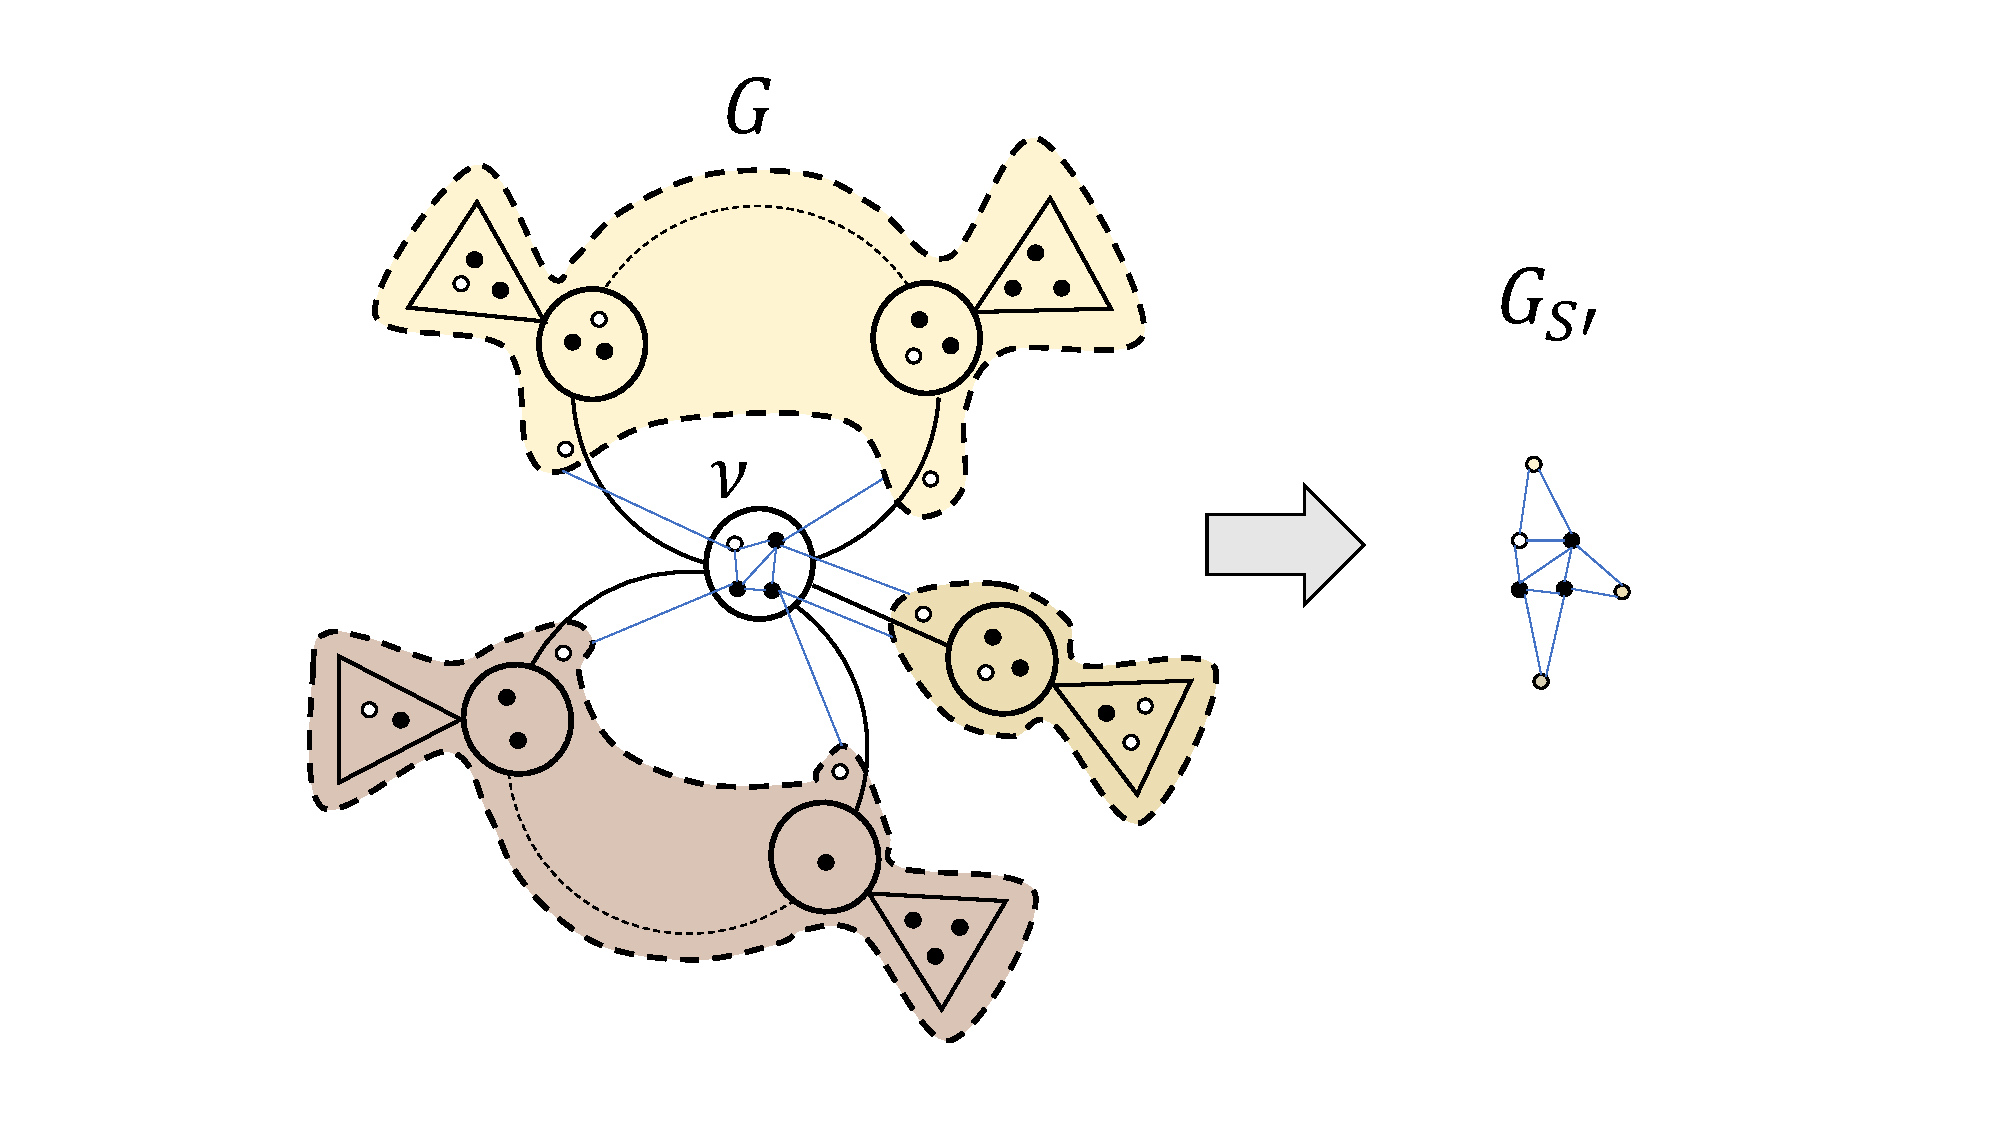
\includegraphics[width=1.0\textwidth]{src/images/image_contraction.pdf}{}
    \caption{Contraction procedure. We only show the vertices of graph, some edges of graph and the skeleton ${\cal H}_S$. Solid vertices belong to steiner set $S$ and hollow vertices are non-steiner vertices. Blue edges denote some of the graph edges.}
    \label{fig:image-contraction}
\end{figure}

Let us focus on cycle $C_i$ for any $i\le j$. Let $e_1$ and $e_2$ be the structural edges in this cycle that are incident on node $\nu$. Let ${\cal W}$ be the strip corresponding to the subbunch formed by these two structural edges. Let $\mathbf s$ and $\mathbf t$ be the source and sink of this strip respectively. Also, assume that $\nu$ is on the side of source. We now state a lemma that states an important property about $G_\nu$.

\begin{lemma}
Let $u$ be a non-terminal unit in ${\cal W}$. Let $u'$ be any unit reachable from $u$ in the direction of ${\mathbf{s}}$. $u'$ will be compressed to the same cycle node as $u$ during the construction of $G_\nu$.
\label{lem:u-u'-in-G-nu}
\end{lemma}
\begin{proof}
Let the proper paths associated with each of $u$ and $u'$ in ${\cal H}_S$ be $P(\nu_1,\nu_2)$ and $P(\nu_3,\nu_4)$ respectively. 
It follows from the construction of ${\cal W}$ that
$P(\nu_1,\nu_2)$ as well as $P(\nu_3,\nu_4)$ will pass through either structural edge $e_1$ or structural edge $e_2$. Without loss of generality,  assume that $P(\nu_1,\nu_2)$ passes through $e_1$. Since both $e_1$ as well as $e_2$ belong to $C_i$ and $P(\nu_1,\nu_2)$ is a proper path, this would imply that it will not pass through $e_2$. Since $u'$ is reachable from $u$, so $P(\nu_3,\nu_4)$ will also have to pass through $e_1$.
It follows from Corollary \ref{th:reachability-cone-proper-path}, that 
$P(\nu_1,\nu_2)$ as well as $P(\nu_3,\nu_4)$ are subpaths of a path, say $P(\nu',\nu'')$, in skeleton
${\cal H}_S$. This combined with the above discussion establishes that $P(\nu',\nu'')$ has the structure shown in Figure \ref{fig:structure-of-p(nu',nu'')}.

Observe that any path in skeleton that passes through a node $\nu$ can intersect at most 2 cycles that are passing though $\nu$. We know that prefix of $P(\nu',\nu'')$ upto $e_1$ pass through $C_i$, so the suffix can pass through exactly one cycle $C_\ell, \ell \not=i$.
Since $\nu_2$ and $\nu_4$ belong to the compressed node of $C_j$. This completes the proof.
\end{proof}


\begin{lemma}
Let $A_i$ be the set of vertices compressed to $c_i$. The cut $(A_i,\bar{A_i})$ represent a Steiner mincut from strip ${\cal W}$.
\end{lemma}
\begin{proof}
Let $U_k$ be the set of non-terminal units in strip ${\cal W}$ such that the proper path to which it is mapped has one end point in cycle $C_k$. We already know that the other end point is in cycle $C_i$ since this unit appears as a non-terminal in the strip. Consider the cut defined by 
$\cup_{k\not=i} U_k \cup {\mathbf{s}}$.
It follows from Lemma \ref{lem:u-u'-in-G-nu} that 
${\cal R}_{\mathbf s}(U_k) \setminus {\mathbf s} = U_k$.
Therefore, $\cup_{k\not=i} U_k \cup {\mathbf{s}}$ is a transversal on ${\cal W}$, and hence is a Steiner mincut.
\end{proof}


% As evident from the results of \cite{DBLP:journals/mp/PicardQ82}, the number of $(u,v)$-mincuts can be exponential for a designated source and sink vertex. The query $Q(u,v,E_y)$ on graph $G$ requires to check if all edges in $E_y$ lie in some $(u,v)$-mincut. This means that we somehow have to check the presence of these edges in all the $(u,v)$-mincuts. The aim of constructing $G_\nu$ is to preserve as many $(u,v)$-mincuts as possible in a smaller compact graph. However, there may be some $(u,v)$-mincuts in $G$ which are missing in $G_\nu$. To circumvent this problem we transform a query $Q(u,v,E_y)$ on $G$ in such a way that it can be answered from the $(u,v)$-mincuts in $G_\nu$ itself.

% {\color{blue} Revised version ends}



% {\color{red} Old version begins}


% In this section, we will discuss the \textit{contraction procedure}, i.e. obtaining $G_\nu$ from graph $G$ and connectivity carcass $\mathfrak{C}_S$. Thereafter, we establish more formally how $G_\nu$ preserves the connectivity of steiner vertices mapped to node $\nu$.

% \subsubsection{Contraction procedure}
% To accomplish the contraction procedure, we define an order on the cycles. The ordering can be done arbitrarily. Since, $G_\nu$ is a quotient graph of $G$ it can be obtained from $G$ by applying certain vertex contractions. We keep all the vertices mapped to node $\nu$ in the skeleton as it is in $G_\nu$ (call them $V_\nu$). We create a vertex corresponding to each cycle (call them cycle vertices) passing through $\nu$ in new graph $G_\nu$. Now, for each vertex mapped to $P(\nu_1,\nu_2)$ (not $P(\nu,\nu)$) the contraction proceeds as follows,
% \begin{itemize}
%     \item If $P(\nu_1,\nu_2)$ does not pass through $\nu$, then it is contracted to the vertex corresponding to the cycle in which this path completely lies,
%     \item if $P(\nu_1,\nu_2)$ has one end point as $\nu$, then it is contracted to the vertex corresponding to the cycle in which its second end-point lies,
%     \item if $P(\nu_1,\nu_2)$ passes through $\nu$ but does not have it as an end-point, the unit is contracted to the cycle vertex corresponding to lesser ordered cycle.
% \end{itemize}

% \noindent
% Let $C_1,C_2,...,C_j$ be the cycles in the skeleton which pass through node $\nu$. Let us focus on cycle $C_i$. Let $e_1$ and $e_2$ be the structural edges in this cycle that are incident on node $\nu$. Let ${\cal W}$ be the strip corresponding to the bunch formed by these two structural edges. Let $\mathbf s$ and $\mathbf t$ be the source and sink of this strip respectively. Also, assume that $\nu$ is on the side of source.

% Let $U_k$ be the set of non-terminal units in this strip such that the proper path to which it is mapped has one end point in cycle $C_k$ (not $\nu$ although). We already know that the other end point is in cycle $C_i$ since this unit appears as a non-terminal in the strip. Let $\mathbf u \in U_i$ be a non-terminal unit. Using \ref{th:reachability-cone-proper-path}, it is evident that all non-terminal units in ${\cal R}_{\mathbf s}(\mathbf u) \setminus {\mathbf s}$ belong to set $U_i$. Overloading the notation, let ${\cal R}_{\mathbf s}(U_k) \setminus {\mathbf s}$ represents the union of ${\cal R}_{\mathbf s}(\mathbf u) \setminus {\mathbf s}$ $\forall\; {\mathbf u}\in U_k$. This simple property leads to the following,

% \begin{equation}
%     \begin{split}
%         \nonumber
%         {\cal R}_{\mathbf s}(U_k) \setminus {\mathbf s} &= U_k \\
%         \implies \bigcup_{k<i}{\cal R}_{\mathbf s}(U_k) \setminus {\mathbf s} &= \bigcup_{k<i} U_k
%     \end{split}
% \end{equation}

% Thus, the set $\bigcup_{k<i} U_k$ forms a closed set in the strip ${\cal W}$. Consider a transversal $(A,{\bar A})$ such that $A$ contains all the units in $\bigcup_{k<i} U_k$ as well as source $\mathbf{s}$. It is evident that $(A,{\bar A})$ is also a steiner mincut.


% % As evident from the results of \cite{DBLP:journals/mp/PicardQ82}, the number of $(u,v)$-mincuts can be exponential for a designated source and sink vertex. The query $Q(u,v,E_y)$ on graph $G$ requires to check if all edges in $E_y$ lie in some $(u,v)$-mincut. This means that we somehow have to check the presence of these edges in all the $(u,v)$-mincuts. The aim of constructing $G_\nu$ is to preserve as many $(u,v)$-mincuts as possible in a smaller compact graph. However, there may be some $(u,v)$-mincuts in $G$ which are missing in $G_\nu$. To circumvent this problem we transform a query $Q(u,v,E_y)$ on $G$ in such a way that it can be answered from the $(u,v)$-mincuts in $G_\nu$ itself.

% {\color{red} Old version ends}

We establish the following lemma which presents the results of Lemma \ref{lem:small-graph-equivalent-S=V} in a more general form.

\begin{lemma} \label{lem:small-graph-equivalent}
Let $G_\nu$ be the graph corresponding to node $\nu$ in skeleton ${\cal H}_S$, obtained from graph $G$ and connectivity carcass $\mathfrak{C}_S$ using the \textit{contraction procedure}. If $u,v \in V_\nu \cap S$,
\begin{enumerate}
    \item For any $(u,v)$-mincut in $G$, there exists a $(u,v)$-mincut in $G_\nu$ that defines the same $2-$partition of set $V_\nu$. Moreover, the value of $(u,v)$-mincut remains same in both $G$ and $G_\nu$.
    \item Let $E' \subset E$ be a set of edges whose endpoints are contracted to different vertices in $G_\nu$. There is a $(u,v)$-mincut in $G$ that cuts all edges in $E'$, if and only if there is a $(u,v)$-mincut in $G_\nu$ that cuts all edges in $E'$.
\end{enumerate}
\end{lemma}
\begin{proof}
Let $c_1,c_2,...,c_j$ be the cycle vertices in $G_\nu$ corresponding to cycles $C_1,C_2,...,C_j$ of skeleton $\mathcal H_S$. It is also known that $\nu$ is part of all these cycles.

Consider $(A_i,\overline A_i)$ to be a cut in $G$ that keeps all vertices contracted to $c_i$ on side $\overline A_i$ and all the other vertices in $A_i$. We have already argued that each of the cuts $(A_i, \overline A_i)$ form a steiner mincut.

Given a $(u,v)$-mincut ${\cal C}=(B,{\bar B})$ that cuts all edges in $E'$ it suffices to construct another $(u,v)$-mincut ${\cal C}'=(B',{\bar B'})$ that cuts all edges in $E'$ and keeps all the vertices of ${\bar A_i}$ on one side $\forall i \in [j]$. It is clear that such a mincut will also be present in $G_\nu$.

For each set $A_i$, where $i\in [j]$ repeat the following procedure. If $B$ keeps ${\bar A_i}$ on one side proceed to next $i$. Otherwise, if $B\cap {\bar A_i}$ (or ${\bar B}\cap {\bar A_i}$) consists of some steiner vertices then replace the $(u,v)$-mincut $(B,{\bar B})$ by $(u,v)$-mincut $({\bar A_i}\cup B,A_i\cap {\bar B})$ (or $(A_i\cap B,{\bar A_i}\cup {\bar B})$) and proceed to next $i$.

It is clear that following the above procedure we eventually get a $(u,v)$-mincut that keeps all the vertices of ${\bar A_i}$ on one side $\forall i \in [j]$. This $(u,v)$-mincut will define the same partition in $V_\nu$. Moreover, it will also cut all edges in $E'$.

The above result also implies that the value of $(u,v)$-mincut in $G$ is same as that in $G_\nu$ for any $u,v \in V_\nu \cap S$. Thus, the other direction of both the proofs are trivial.
\end{proof}

Again, the above lemma implies that a query $Q(u,v,E')$ on $G$ will produce the same outcome on $G_\nu$ provided that all edges in $E'$ have distinct end points in $G_\nu$. Similar to the base case, we use the notion of query transformation to deal with the  edges whose end point are contracted to single vertex in $G_\nu$. Thus, we arrive at the following lemma that presents our key insight in the most concise form.

\begin{lemma} \label{lem:edge-correspondence}
Let $u,v \in S$ mapped to same node $\nu$ in skeleton $\mathcal H_S$ corresponding to graph $G$ and steiner set $S\subseteq V$. For a given set of edges $E_y$ emanating from a given vertex $y$ in $G$, there exists a set of edges $E_{y'}$ emanating from a vertex $y'$ in $G_\nu$ such that $E_y$ lies in a $(u,v)$-mincut in $G$ if and only if $E_{y'}$ lies in a $(u,v)$-mincut in $G_\nu$. Set of edges $E_{y'}$ can be obtained from $E_y$ given flesh $\mathcal F_S$ and skeleton $\mathcal H_S$ in time linear in the size of flesh.
\end{lemma}

\begin{proof}
First of all we consider the case when $y$ is mapped to $\nu$. In this case, all the edges of $E_y$ are also present in $G_\nu$. Using Lemma \ref{lem:small-graph-equivalent}(ii), it is clear that the proposition holds taking $y'=y$ and $E_{y'}=E_y$.

% Now, consider the case when $y$ is contracted to some cycle node $c$ in $G_\nu$. Assume that cycle node $c$ corresponds to cycle $C$ in the skeleton ${\cal H}_S$. Consider $(A,{\bar A})$ to be the steiner mincut in graph $G$ such that ${\bar A}$ consists of all the vertices contracted to cycle node $c$. Also consider a $(u,v)$-mincut $(B,{\bar B})$ that cuts all edges in $E_y$. Based upon whether the cut $(B,{\bar B})$ $S-$crosses the cut $(A,{\bar A})$ one of the cases from Lemma \ref{lem:crossing-and-non-crossing-steiner-mincut} may arise. Without loss in generality, it can be assumed that $B\cap {\bar A}$ contains atleast a steiner vertex. It can be observed that in either of the cases ${\bar A}\cap B$ defines a steiner mincut. Since, this steiner mincut cuts all edges in $E_y$, they must be in the same side of the inherent partition of $y$. 

% Now, consider the case when $y$ is contracted to some cycle node $c$ in $G_\nu$. Assume that cycle node $c$ corresponds to cycle $C$ in the skeleton ${\cal H}_S$. Consider $(A,{\bar A})$ to be the steiner mincut in graph $G$ such that ${\bar A}$ consists of all the vertices contracted to cycle node $c$. Also consider a $(u,v)$-mincut $(B,{\bar B})$ that cuts all edges in $E_y$. Based upon whether the cut $(B,{\bar B})$ $S-$crosses the cut $(A,{\bar A})$ one of the cases from Lemma \ref{lem:crossing-and-non-crossing-steiner-mincut} may arise. Without loss in generality, it can be assumed that $B\cap {\bar A}$ contains atleast a steiner vertex. It can be observed that in either of the cases ${\bar A}\cap B$ defines a steiner mincut. Since, this steiner mincut cuts all edges in $E_y$, they must be in the same side of the inherent partition of $y$. 

Consider $(A,{\bar A})$ to be the steiner mincut in graph $G$ such that ${\bar A}$ consists of all the vertices contracted to cycle node $c$.

Let unit mapped to node $\nu$ be $U$ and thus $u,v\in U$. Consider \textit{any} steiner unit $U_1 \notin A$ mapped to node $\nu_1$. Construct the strip ${\cal W}$ containing all steiner mincuts separating $U$ from $U_1$. If there exists any $(u,v)$-mincut $B$ that cuts all edges in $E_y$, then all edges in $E_y$ must appear in the strip. This is because if $U_1 \in B$ (wlog) then ${\bar A}\cap B$ must be a steiner mincut (from Lemma \ref{lem:crossing-and-non-crossing-steiner-mincut} (i)) separating $U_1$ from $U$ and also cutting all edges in $E_y$.

Using Lemma \ref{lem:reachability-cone-u-v-mincut}, we can obtain another set of edges $E_{y'}$ that have one end point in ${\bar A}$ and other end point in $A$, and also satisfy the property that all edges in $E_y$ lie in some $(u,v)$-mincut ${\cal C}$ in $G$ if and only if all edges in $E_{y'}$ lie in some $(u,v)$-mincut ${\cal C}'$ of $G$. Moreover, using \ref{lem:small-graph-equivalent} (ii) we can argue that this can happen if and only if there exists a $(u,v)$-mincut in $G_\nu$ that cuts all edges in $E_{y'}$. Final thing to observe is that all edges in $E_{y'}$ do emanate from a single vertex $y'=c$ in graph $G_\nu$. This completes the proof for first part.

% Let $y$ be a stretched unit in the skeleton. Assume the proper path to which it is mapped in skeleton ${\cal H}_S$ be $P(\nu_1,\nu_2)$. Consider the paths $(\nu,\nu_1)$,$(\nu,\nu_2)$ and $(\nu_1,\nu_2)$ in the tree ${\cal T}({\cal H}_S)$. Atleast one of the paths $(\nu,\nu_1)$ or $(\nu,\nu_2)$ must intersect the path $(\nu_1,\nu_2)$. Let $(\nu,\nu_1)$ be one such path. Consider the strip consisting of all mincuts between node $\nu_1$ and node $\nu$. Since, $y$ appears as a non-terminal in this strip, it is clear that all edges in $E_y$ must be present in this strip. Moreover,$A$ will appear as a transversal in this strip. Using Lemma \ref{lem:reachability-cone-u-v-mincut}, we can obtain another set of edges $E_{y'}$ that have one end point in ${\bar A}$ and other end point in $A$, and also satisfy the property that all edges in $E_y$ lie in some $(u,v)$-mincut ${\cal C}$ in $G$ if and only if all edges in $E_{y'}$ lie in some $(u,v)$-mincut ${\cal C}'$ of $G$. Moreover, using \ref{lem:small-graph-equivalent} (ii) we can argue that this can happen if and only if there exists a $(u,v)$-mincut in $G_\nu$ that cuts all edges in $E_{y'}$. Final thing to observe is that all edges in $E_{y'}$ do emanate from a single vertex $y'=c$ in graph $G_\nu$. This completes the proof for first part.

% Let $y$ is a terminal unit and mapped to node $\nu_1$. We can again accomplish the procedure by constructing the strip ${\cal W}$ consisting of all mincuts between node $\nu_1$ and $\nu$. However, the explanation is slightly different in this case. Assume that $B$ does not $S-$cross $A$. In this case, all the units in ${\bar A}\cap {\bar B}$ are stretched units. Thus, $y$ must lie in ${\bar A}\cap B$. Clearly, ${\bar A}\cap B$ is a steiner mincut that separates $y$ from $\nu$. Thus, all edges in $E_y$ must be present in the strip ${\cal W}$. Same observation can be made in the case when $B$ $S-$crosses $A$. If all edges in $E_y$ are present in ${\cal W}$, the remaining proof is same as above. Now, it is quite possible that all edges in $E_y$ are not present in strip ${\cal W}$. We have already shown that this implies that all edges in $E_y$ cannot lie in any $(u,v)$-mincut. The lemma trivially holds in this case as well.


% Observe the proper path to which any edge in $E_y$ is mapped in the skeleton. Foremost property to observe is that all these proper paths must be extendable to a bigger proper path which can intersect cycle $C$ at atmost one structural edge. It can be shown that all edges in $E_y$ must be mapped to a proper path that intersects cycle $C$ at a structural edge. 

% Consider the case when $B$ does not $S-$crosses $A$. It is clear that the steiner mincuts $A$ and $A\cap {\bar B}$ define the same $2-$partition of the steiner set and hence, belong to same bunch. Since the cut $(A,{\bar A})$ is induced by two structural edges of $C$ incident on $\nu$ (say $e_1,e_2$), the cut $(A\cap {\bar B},{\bar A}\cup B)$ must be induced by the same two structural edges. This means that all the edges in $E_y$ must be mapped to a proper path that intersects cycle $C$ at structural edges $e_1$ or $e_2$. Consider the other case when $B$ $S$-crosses $A$. It this case, from Lemma \ref{lem:crossing-and-non-crossing-steiner-mincut} (ii) it follows that all the three cuts $A$, ${\bar A}\cap B$ and ${\bar A}\cap {\bar B}$ are steiner mincuts and define a partition on the vertex set $V$. Moreover, $A$ is induced by two structural edges $(e_1,e_2)$ in $C$  incident on $\nu$. Using Lemma \ref{lem:3-partition-from-cycle}, we can argue that the other two cuts also arise from same cycle. Let $e_3$ be the other structural edge in the cycle $C$, such that cuts  ${\bar A}\cap B$ and ${\bar A}\cap {\bar B}$ are induced by edges $(e_1,e_3)$ and $(e_2,e_3)$ respectively. Since, all edges in $E_y$ are cut by both these cuts, it is clear that all edges in $E_y$ must be mapped to proper paths which intersects cycle $C$ at structural edge $e_3$.

% Henceforth, we assume that-
% ~(i) $E_y$ lie in same inherent partition of $y$ in flesh ${\cal F}_S$, and
% ~(ii) all edges in $E_y$ are mapped to proper paths which intersect cycle $C$ at structural edges $e_1,e_2$ or some other structural edge $e_3$ of skeleton ${\cal H}_S$. Violating any of the above conditions implies that there is no $(u,v)$-mincut that can cut all edges in $E_y$.

% Consider $e$ to be one of the structural edge of cycle $C$ to which all edges in set $E_y$ are mapped. Let $\mu$ ($\neq \nu$) be one end point of structural edge $e$. Consider the $(\pi^{-1}(\mu),\pi^{-1}(\nu))$ strip storing all mincuts separating vertices mapped to $\mu$ from those mapped to $\nu$. We know that cut $A$ will appear as a transversal in this strip. Moreover, $y$ must appear outside this transversal in the strip. Using Lemma \ref{lem:reachability-cone-u-v-mincut}, we can obtain another set of edges $E_y'$ that have one end point in ${\bar A}$ and other end point in $A$, and also satisfy the property that all edges in $E_y$ lie in some $(u,v)$-mincut ${\cal C}$ in $G$ if and only if all edges in $E_{y'}$ lie in some $(u,v)$-mincut ${\cal C}'$ of $G$. Moreover, using \ref{lem:small-graph-equivalent} (ii) we can argue that this can happen if and only if there exists a $(u,v)$-mincut in $G_\nu$ that cuts all edges in $E_{y'}$. Final thing to observe is that all edges in $E_{y'}$ do emanate from a single vertex $y'=c$ in graph $G_\nu$. This completes the proof for first part.

Obtaining the edges $E_{y'}$ can be done by
~(i) constructing the strip ${\cal W}$ storing all steiner mincuts separating $U$ and $U_1$,
~(ii) computing multiple reachability cones in this dag to obtain $E_{y'}$. Each of these procedures can be carried out in time linear to the size of flesh graph ${\cal F}_S$.
\end{proof}



Using \ref{lem:edge-correspondence}, it is easy to observe that query $Q(u,v,E_y)$ in $G$ is equivalent to the query $Q(u,v,E_{y'})$ on $G_\nu$. We will use this construction of $G_\nu$ to build our ${\cal O}(m)$ size data structure. Furthermore, it will be shown that the query procedure on this data structure which uses multiple query transformations takes ${\cal O}(\min(m,nc_{uv}))$ time in total.